% Created 2021-11-09 Tue 14:50
% Intended LaTeX compiler: pdflatex
\documentclass[11pt]{article}
\usepackage[utf8]{inputenc}
\usepackage[T1]{fontenc}
\usepackage{graphicx}
\usepackage{grffile}
\usepackage{longtable}
\usepackage{wrapfig}
\usepackage{rotating}
\usepackage[normalem]{ulem}
\usepackage{amsmath}
\usepackage{textcomp}
\usepackage{amssymb}
\usepackage{capt-of}
\usepackage{hyperref}
\usepackage{minted}
\usepackage[utf8]{inputenc}
\usepackage[dvipsnames]{xcolor}
\usepackage{tikz}
\usepackage{pdfpages}
\usepackage[, germanb]{babel}
\usepackage{listings}
\usepackage[]{babel}
\usepackage[dvipsnames]{xcolor}
\usepackage{courier}
\usepackage{listings}
\usepackage{textcomp}
\usepackage{gensymb}
\author{Jakob Klemm}
\date{}
\title{Actaeon}
\hypersetup{
 pdfauthor={Jakob Klemm},
 pdftitle={Actaeon},
 pdfkeywords={},
 pdfsubject={},
 pdfcreator={Emacs 28.0.50 (Org mode 9.4.4)}, 
 pdflang={Germanb}}
\begin{document}

\maketitle
\tableofcontents

\newpage

\section{Einführung}
\label{sec:org5129707}
Dieses Dokument soll ohne grosse Umschreibungen und ohne
Dramatisierungen einen Einblick in die Konzepte und Entscheidungen und
Systeme bieten, welche schlussendlich zur \texttt{actaeon} Bibliothek geführt
haben. Es ist ebenfalls wichtig zu verstehen, dass dieses Dokument
sich lediglich auf die, im Rahmen der Maturarbeit entstandenen
Projekte beschränkt, es handelt sich hier nicht um eine komplette
Einführung in dezentrale Datensysteme, allerdings existieren genügend
Quellen für grundlegendere Informationen\footnote{Orion Wiki - Distributed Systems, Jakob Klemm. \url{https://orion.jeykey.net/distributed\_systems.pdf}}. Für das
schlussendliche Produkt wurde die \texttt{Rust}-Programmiersprache verwendet,
welche ebenfalls nicht hier erklärt werden soll.
\section{Projekte}
\label{sec:org7fc11a6}
Nachdem die zentralen Problemen definiert wurden, ist es an der Zeit,
andere Projekte zu analysieren um herauszufinden, ob die Probleme
bereits vollständig oder zumindest teilweise gelöst wurden.\\

\noindent Zwar wurden viele Probleme und Gefahren angesprochen,
\texttt{Engine: Orin} soll sich allerdings nur auf die folgenden beiden Aspekte
fokussieren:
\begin{itemize}
\item ein Nachrichtensystem zum Senden und Lenken der einzelnen
Nachrichten.
\item ein System zur Verarbeitung der einzelnen Nachrichten.
\end{itemize}
Dementsprechend sollen auch andere Projekte, die sich mit diesen
beiden Aspekten analysiert werden. Um aber die Wahl der Projekte
richtig zu verstehen, muss man die Vision hinter \texttt{Engine: Orion} im
Blick behalten. Denn es wird schnell klar, dass es für alle
beschriebenen Probleme entweder temporäre Lösungen oder einzelne
Projekte zur Umgehung der Probleme gibt. Daneben existieren auch
grundlegendere Neuentwicklungen bekannter Systeme, welche einzelne
Probleme lösen, meist aber andere Ziele haben. Was allerdings kein
bekanntes Projekt umzusetzen versucht, ist nicht nur die grundlegende
Neuentwicklung zentraler Systeme zur Behebung bekannter Probleme,
sondern dazu noch die nahtlose Integration der einzelnen Komponenten
für ein durchgehend integriertes, zusammenspielendes System.\\

\noindent Da ein solches Projekt nicht öffentlich existiert, müssen
stattdessen die einzelnen Probleme und deren Lösungsversuche
angeschaut werden. Dafür wird grundlegend in zwei zentrale Komponenten
unterschieden. Die Integration der beiden Teile soll hier nicht
besprochen werden, da diese sich hauptsächlich in der Umsetzung zeigt.
\subsection{Kademlia}
\label{sec:org710a836}
Wie geht man also gegen die totale Abhängikeit von Internetanbietern
und zentralen Routern vor?\\
Man kann ja nicht einfach seine eigenen Router aufsetzen und einen
alternativen Dienst anbieten. Neben den technischen Schwierigkeiten
würde ein solcher Schritt auch überhaupt nichts das eigentliche
Problem bekämpfen.\\

\noindent Der Trick, der bei Systemen wie \texttt{Kademlia} verwendet wird, ist
es, Router vollständig zu eliminieren. Dies ist möglich, indem jedes
Mitglied des Netzwerks neben seinen normalen Funktionen gleichzeitig
auch noch als Router agiert. Strenggenommen werden in \texttt{Kademlia} Router
also nicht wirklich eliminiert, lediglich zentrale Router fallen
weg.\\

\noindent In einem früheren Abschnitt wurden die Probleme der
\emph{Zentralrouter} bereits angesprochen. Wenn jetzt aber jedes Mitglied in
einem Netzwerk plötzlich als Router agiert und es keine zentrale
Instanz gibt, träfe die Problematik der \emph{Zentralrouter} plötzlich auf
alle Server zu. Genau da kommt \texttt{Kademlia} ins Spiel. Aber was genau ist
\texttt{Kademlia} eigentlich?\\

\noindent Laut den Erfindern, \emph{Petar Maymounkov} und \emph{David Mazières},
ist es
\begin{center}
ein Peer-to-peer Nachrichten System basierend auf XOR-Metrik.\footnote{Kademlia: Whitepaper:
\url{https://pdos.csail.mit.edu/\~petar/papers/maymounkov-kademlia-lncs.pdf},
heruntergeladen am: 30.05.2020.}
\end{center}
Was genau bedeutet das und wie lässt sich eine \texttt{XOR}-Metrik für
verteilte Datensysteme einsetzen?\\

\noindent Da die einzelnen Server nicht in der Lage sind,
Informationen über das komplette Netzwerk zu speichern oder zu
verarbeiten, funktionieren \texttt{Kademlia}-Systeme grundlegend anders.
Anstelle der hierarchischen Anordnung der Router ist jedes Mitglied
eines Systems gleichgestellt. dabei kümmert sich jedes Mitglied auch
nicht um das komplette System, sondern nur um sein direktes Umfeld.
Während dies für kleinere Systeme gut funktioniert und vergleichbare
Geschwindigkeiten liefert, skaliert es nicht so einfach für grosse
Systeme. Genau dafür gibt es die \texttt{XOR}-Metrik.
\subsubsection{Distanz}
\label{sec:org78c7914}
Die \texttt{XOR}-Funktion, die in der Informatik an den verschiedensten
Orten auftaucht, wird verwendet, um die Distanz zwischen zwei
Zahlen zu berechnen. Die Zahlen repräsentieren dabei Mitglieder
im Netzwerk und sind je nach Variante im Bereich
\(0..2^{160}\)(\emph{20 Bytes}) oder \(0..2^{256}\)(\emph{32 Bytes}). Mit einem
so grossen Bereich lässt sich auch das Problem der limitierten
\texttt{IP-Adressen} lösen. Auch wenn es kein tatsächlich unlimitiertes
System ist, so gibt es doch mehr als genug Adressen.\\

\noindent Wenn mit \texttt{XOR}-Funktionen einfach die Distanz zwischen
zwei Zahlen berechnet wird, stellt sich die Frage, wieso nicht
einfach die Differenz verwendet wird. Um dies zu beantworten,
muss man sich die Eigenschaften der \texttt{XOR}-Funktion etwas genauer
anschauen:

\begin{enumerate}
\item \(xor(x, x) = 0\): Das Mitglied mit seiner eigenen Adresse ist
zu sich selbst am nächsten. Mitglieder werden hier als Namen
für Server in einem \texttt{Kademlia}-System verwendet.
\item \(xor(x, y) > 0\) wenn \(x \neq y\): Die Funktion produziert nie
negative Zahlen und nur mit zwei identischen Parametern kann
man \(0\) erhalten.
\item \(xor(x, y) = xor(y, x)\): Die Reihenfolge der Parameter spielt
keine Rolle.
\item \(xor(x, z) \leq xor(x, y) + xor(y, z)\): Die direkte Distanz
zwischen zwei Punkten ist am kürzesten oder gleich kurz wie
die Distanz mit einem zusätzlichen Schritt dazwischen, also
einem weiteren Sprung im Netzwerk.
\item Für ein gegebenes \(x\) und eine Distanz \(l\) gibt es nur
genau ein \(y\) für das \(xor(x, y) = l\) gilt.
\end{enumerate}

\noindent Aber wieso genau funktioniert dies? Wieso kann man \texttt{XOR}, eine
Funktion zur Berechnung der Bit-Unterschiede in zwei Binärzahlen,
verwenden, um die Distanz zwischen zwei Punkten in einem verteilten
Datensystem zu berechnen?\\

\noindent Um dies zu verstehen, hilft es, sich das System als
umgekehrten Baum vorzustellen. Untergeordnet zum zentralen Punkt zu
oberst stehen alle Mitglieder im System. Mit jeder weiteren Abzweigung
zweier Teilbäume halbiert sich die Anzahl. Man wählt am einfachsten
zwei Abzweigungen pro Knoten, da sich damit die Werte direkt als
Binärzahlen darstellen lassen, wobei jeder Knotenpunkt einfach eine
Stelle in der langen Kette aus \(0\) oder \(1\) darstellt. Der ganze
Baum sieht dann wie folgt aus\footnote{Wikipedia: Kademlia \url{https://en.wikipedia.org/wiki/Kademlia},
heruntergeladen am: 30.05.2020.}:

\begin{center}
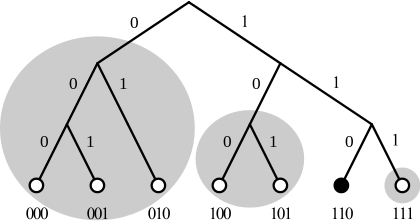
\includegraphics[width=.9\linewidth]{tree.png}
\captionof{figure}{Beispielhafte Darstellung eines einfachen Kademlia-Systems}
\end{center}

\noindent Mit dieser Sicht auf das System beschreibt die \texttt{XOR}-Funktion
die Anzahl der unterschiedlichen Abbiegungen im Baum und somit die
Distanz. Zwar mag es auf den ersten Blick nicht intuitiv wirken, wieso
man \texttt{XOR} anstatt einfach der Differenz verwendet, allerdings
funktioniert die Funktion mit Binärzahlen in einem solchen Baum
einiges besser.
\subsubsection{Routing-Table}
\label{sec:orgfb01e12}
In einem \texttt{Kademlia}-System hat jedes Mitglied eine gewisse Anzahl
anderer Mitglieder, mit denen es sich verbunden hat. Da \texttt{Kademlia} ein
sehr umfangreiches, kompliziertes Protokoll und System beschreibt,
sollen hier nur einige zentrale Funktionen besprochen werden, die für
diesen ersten Prototypen von \texttt{Engine: Orion} relevant sind. Besonders
beim \texttt{Routing Table} lassen sich einige Abschnitte weglassen, welche
zwar für die Optimierung und Skalierung eines Systems wichtig,
allerdings für das Analysieren eines einfachen, kleinen Systems wie
\texttt{Engine: Orion} irrelevant sind.\\

\noindent Einfach formuliert speichert der \texttt{Routing Table} die
verbundenen Mitglieder. Eine eingehende Nachricht wird dann mithilfe
dieser Liste, sowie der \texttt{XOR}-Metrik ans richtige Ziel geschickt. Um das
System zu optimieren und die Anzahl der benötigten Sprünge klein zu
halten, wird ein spezielles System verwendet, um zu entscheiden,
welche Mitglieder im \texttt{Routing-Table} gespeichert werden sollen:

\begin{enumerate}
\item Sehr nahe an sich selbst (in der obigen Darstellung also:
wenige Sprünge im Baum) werden alle Mitglieder gespeichert.
\item Je weiter weg sich die Mitglieder befinden, desto weniger
werden gespeichert.
\end{enumerate}

\noindent Die optimale Anzahl der gespeicherten Mitglieder hängt von
den Zielen und Ansprüchen an das System ab. Grundlegend muss man die
Frage beantworten, mit wie vielen Unterbäumen Verbindungen gehalten
werden sollen. Zwar mag dies etwas abstrakt wirken, es lässt sich aber
mit dem eben eingeführten Modell eines umgekehrten Baumes gut
erklären:
\begin{itemize}
\item In der obersten Ebene trennt sich der Baum in zwei vollständig
getrennte Teile, was sich mit jeder weiteren Ebene wiederholt.
\item Die einzige Möglichkeit vom einen \emph{Ende} des Baums zum anderen
zu kommen, ist über den obersten Knoten. Um also in die andere
Hälfte zu kommen, braucht man mindestens eine Verbindungsstelle
in der anderen Hälfte.
\item Deshalb braucht ein \texttt{Routing-Table} nicht nur kurze
Verbindungen zu nahen Punkten, sondern auch einige wenige
Verbindungen zu Mitgliedern in der anderen Hälfte.
\item Mit nur einer weit entfernten Adresse hat man eine Verbindung
in \emph{eigene} und die \emph{andere} Hälfte. Hat man zwei solche
Verbindungen auf die andere Seite hat man schon Verbindungen in
jeden Viertel des Baumes.
\item Man muss also entscheiden, wie fein man die andere Hälfte
aufteilen will. (Eine genaue Unterteilung bedeutet wenige
Sprünge aber grosse \texttt{Routing-Tables}, eine grobe Unterteilung
genau das Umgekehrte).
\end{itemize}

\noindent Zwar hat ein vollständiges \texttt{Kademlia}-System noch
komplexere Elemente, wie \texttt{k-Buckets}, welche den \texttt{Routing-Table}
optimieren, allerdings sind diese für die grundlegende
Funktionsweise des Systems irrelevant.\\

\noindent Die dynamische Regulation des \texttt{Routing-Tables} muss
allerdings noch erwähnt werden:
\begin{itemize}
\item Sobald die definierte Maximalgrösse erreicht ist, werden keine
neuen Verbindungen akzeptiert.
\item Zwar können existierende Einträge durch Neue ersetzt werden,
allerdings werden dabei nicht alte, sondern inaktive Einträge
entfernt. Für ein \texttt{Kademlia}-System werden also auch Mechanismen
benötigt, um die Zustände aller Verbindungen periodisch zu
überprüfen.
\end{itemize}
\subsection{BitTorrent}
\label{sec:org1786e21}
Dezentralisierung hat viele Vorteile und muss langfristig
flächendeckend eingesetzt werden. Aktuell sind die meisten
Industrien und Produkte noch nicht so weit. Trotzdem gibt es
einige Anwendungen und Gruppen bei denen solche Systeme bereits
seit Jahren Verwendung finden.\\

\noindent Beispielsweise im Zusammenhang mit \emph{(mehr oder weniger
legalen)} Verbreiten von Materialien wie Filmen oder Musik wird
eines der grössten global verteilten Systeme eingesetzt. Natürlich
gibt es hunderte von verschiedenen Programmen, Ideen und
Umsetzungen, wobei die meisten Nachfolger von \texttt{Napster} sind.\\

\noindent Im preisgekrönten Film \emph{The social network} erhält man
Einblick in den Lebensstil von \texttt{Sean Parker}, einem der Gründer von
\texttt{Napster}. Es mag überraschen, wie jemand wie Parker, der nur wenige
Jahre zuvor mit \texttt{Napster} die komplette Musikindustrie in Unruhe
gebracht hatte, eine so zentrale Rolle in \texttt{Facebook}, einem der
zentralisiertesten Megaunternehmen der Welt, einnehmen konnte.\\

\noindent Auch wenn es noch nicht \emph{vollständig} dezentralisiert ist,
erlaubte es \texttt{Napster} Nutzern, Musik über ein automatisiertes System
mit anderen Nutzern zu teilen und neue Titel direkt von den
Geräten anderer Nutzer herunterzuladen. Dabei gab es allerdings
immer noch einen zentralen Server, der die Titel sortierte und
indizierte. \\
\texttt{Napster} musste am Ende abgeschaltet werden, nachdem die Klagen der
Musikindustrie zu belastend wurden. Auch wenn das Produkt
abgeschaltet wurde, liess sich nichts mehr gegen die Idee
unternehmen.\\

\noindent Über viele Iterationen und Generationen hinweg wurden
die verteilten Systeme immer weiter verbessert, jegliche zentrale
Server entfernt und in die Hände immer mehr Nutzer gebracht. Heute
läuft ein Grossteil des Austauschs über \texttt{BitTorrent}.

\noindent \texttt{BitTorrent} baut auf der gleichen grundlegenden Idee wie
\texttt{Napster} auf: Nutzer stellen ihren eigenen Katalog an Medien zur
Verfügung und können Inhalte von allen anderen Mitgliedern im
System herunterladen. Anders als \texttt{Napster} gibt es bei \texttt{BitTorrent}
keine zentrale Komponente, stattdessen findet selbst das
Indizieren und Finden von Inhalten dezentralisiert statt\footnote{BitTorrent: Mainline DHT:
\url{https://www.cs.helsinki.fi/u/lxwang/publications/P2P2013\_13.pdf},
heruntergeladen am: 4.06.2020.}.
Dafür wird über das \texttt{Kademlia}-System aktiv bekannt gegeben, wer
welche Inhalte zur Verfügung stellt, wobei einzelne Mitglieder
speichern können, wer die gleichen Inhalte anbietet. Neben
Dezentralisierung und Sicherheit lassen sich über \texttt{BitTorrent}
tatsächlich gute Geschwindigkeiten erreichen, da sich Inhalte von
mehreren Anbietern gleichzeitig herunterladen lassen. Da es sich
bei \texttt{BitTorrent} eigentlich um ein grosses Dateisystem handelt,
lassen sich direkt die \texttt{SHA1}-Hashwerte der Inhalte als
\texttt{Kademlia}-Adressen verwenden.
\subsection{Tox}
\label{sec:orgbcd0e0d}
Im Sommer 2013 veröffentlichte Edward Snowden schockierende
Geheimnisse über massive Spionage Prgogramme der NSA, mit welchen
nahezu aller digitaler Verkehr, ohne Rücksicht auf Datenschutz oder
Privatsphären mitgelesen, ausgewertet und gespeichert wurde. Nahezu
jede Person mit war betroffen und das genaue Ausmass ist bis heute
noch schwer greiffbar. Vielen wurde aber klar, dass sichere,
verschlüsselte Kommunikation nicht mehr nur etwas für Kriminelle und
\emph{Nerds} war, sondern dass jeder Zugang zu verschlüsselter, sicherer und
dezentraler Kommunikation haben sollte. In einem Thread auf 4chan
kamen wurden viele dieser Bedenken gesammelt und es kam die Idee auf,
selbst eine Alternative zu herrkömmlichen Chat Programmen wie Skype zu
entwickeln. Aus dieser Initiative heraus entstand \texttt{Tox}, wobei die Namen
vieler der ursprünglichen Entwickler bis heute unbekannt sind. Damals
war das Ziel die Entwicklung einer sicheren Alternative zu Skype zu
entwicklen, allerdings hat sich der Umfang des Projekts inzwischen
ausgeweitet. Im Zentrum der Arbeiten steht das \texttt{Tox Protocol}, welches
dann von verschiedenen, unabhängigen Programmen umgesetzt wird. Zwar
ist Chat weiterhin eine zentrale Funktion, es wird aber auch Video-
und Audiokommunikation sowie Filesharing gearbeitet.\\

\noindent Basierend auf der bekannten \texttt{NaCl}-Bibliothek\footnote{\texttt{NaCl} Verschlüsselungs Bibliothek:
\url{https://nacl.cr.yp.to/}, heruntergeladen am: 22.09.2021.} wird die
gesamte Kommunikation über das \texttt{Tox Protocol} \footnote{Tox Protokoll Spezifikationen:  
\url{https://toktok.ltd/spec.html}, heruntergeladen am: 22.09.2021.} zwingend End- zu
Endverschlüsselt. Intern wird ein dezentrales Routing System basierend
auf Kademila verwendet, mit welchem Kontakt zwischen Nutzern
(Freunden) aufgebaut wird. Während im Kademila Whitepaper Addressen
mit einer Länge von 20 Bytes definiert werden, nutzt \texttt{Tox} 32 Bytes.
Dies vereinfacht die Verschlüsselung stark, da \texttt{NaCl} Schlüssel
verwendet, welche ebenfalls 32 Bytes lang sind. Nebst der eingesparten
Verhandlung von Schlüsseln und der zusätzlichen Kommunikation bindet
diese Idee die Verschlüsselung direkt stärker in das Routing System
ein, denn es werden keine zusätzlichen Informationen zum Verschlüsseln
einer Nachricht gebraucht und sie kann direkt mit der Addresse des
Ziels verschlüsselt werden.\\

\noindent Es ist allerdings wichtig festzustellen, dass \texttt{Tox} Kademila
lediglich als Router verwendet. Kontakt zwischen zwei Nutzern wird
komplett dezentral hergestellt, sobald diese sich allerdings gefunden
haben wechseln zu einer direkten Kommunikation über UDP. Zwar erlaubt
diese zweiteilung der Kommunikation schnellen Datenverkehr sobald sich
zwei Nutzer gefunden haben (so ist beispielsweise Video- und
Audiokommunikation möglich), es kommen aber auch einige neue Probleme
auf:
\begin{itemize}
\item Anders als beispielsweise im Darknet über das Onion-Routing von
Aussen klar erkennbar, mit wem jemand kommuniziert. Natürlich ist
der Inhalt weiterhin verschlüsselt, aber ein solches System setzt in
erster Linie auf Sicherheit und Geschwindigkeit und nicht auf
Anonymität.
\item Auch muss man bedenken, dass nicht jedes Gerät im Internet in der
Lage ist direkte Verbindungen mit jedem anderen Gerät aufzubauen.
Besonders Firewalls können schnell zu Problemen führen. Um den
Aufwand für die Nutzer zu minimieren wird \texttt{UDP hole punching} \footnote{Wikipedia: UDP Hole punching:  
\url{https://en.wikipedia.org/wiki/Hole\_punching\_(networking)},
heruntergeladen am: 24.09.2021.}
verwendet, allerdings existieren auch dafür gewisse Kriterien und
Probeleme.
\end{itemize}

\noindent Das \texttt{Tox Protocol} bietet eine einheitliche Spezifikation mit
der eine grosse Auswahl an Problemen gelöst werden können. Wer eine
sichere, dezentrale Alternative zu Whatsapp sucht könnte an \texttt{Tox}
gefallen finden. Seit einigen Jahren gibt es aber Bedenken über die
Sicherheit und aktuelle Richtung des Projekts, sowie Berichte von
internen Konflikten, besonders im Zusammenhang mit Spendengeldern.
\section{Architektur}
\label{sec:org35a8e07}
In diesem Kapitel sollen einige der zentralen Konzepte und
Entscheidungen erläutert werden, welche schlussendlich zur
\texttt{Actaeon}-Applikation geführt haben.
\subsection{Verschlüsselung}
\label{sec:org3133587}
Zwar ist es bei weitem nicht, dass moderne dezentrale Systeme das
Internet oder ein ähnliches Austauschsystem als Grundlage verwenden,
allerdings ist dies in nahezu allen Fällen, besonders bei den
beliebten und weit verbreiteten Fällen. Das Internet ist für fehlende
Sicherheit und Gefahren bekannt, daher ist es von Nöten, dass sich
jede Applikation selbst um Verschlüsselungen und Sicherheit kümmert.
Allerdings ist es wichtig, \emph{die passende Verschlüsselung} zu wählen.
Hier wird nun ein Ansatz beschrieben, welcher sich besonders gut für
gewisse \texttt{Kademlia}-inspirierte Systeme eignet. Dieser Ansatz beruht auf
der Verschlüsselungs-Bibliothek \texttt{NaCl}, beziehungsweise deren modernen
Abzweig \texttt{libsodium}. Während klassische Verschlüsselungsmethoden sehr
lange Schlüssel benötigen, gibt es gewisse Kombinationen von
Algorithmen, welche mit sehr kurzen Schlüsseln Sicherheit
gewährleisten können. Besonders geht es dabei um
\texttt{curve25519xsalsa20poly1305}, einer Kombination aus den Algorithmen
\texttt{Curve25519}, \texttt{Salsa20} und \texttt{Poly1305}. Während das innere Zusammenspiel
dieser Algorithmen sehr komplex wirken mag, ist das Resultat ein
Algorithmus, wessen Schlüssel jeweils nur eine Länge von \emph{32 bytes}
haben.\\

\noindent Eigentlich beschreibt \texttt{Kademlia} Adressen mit einer Länge von
\emph{160 bits} oder \emph{20 bytes}, allerdings ist es ohne grosse Probleme
möglich, die Adressen Länge auf \emph{32 bytes} zu verlängern. Dies erlaubt
es uns, die Verschlüsselung und das Adresssystem direkt miteinander zu
verbinden. Das mag auf den ersten Blick etwas umständlich und
unlogisch wirken, es erlaubt allerdings, ohne weitere Operationen
verschlüsselte Nachrichten an einen Nutzer zu schicken, wobei
lediglich dessen Adresse bekannt sein muss. Insgesamt fällt damit viel
Komplexität weg und macht das erstellen, verifizieren und finden von
Adressen viel einfacher.
\subsection{PubSub}
\label{sec:org81ed48f}
Ein einfaches, aber vielseitig einsetzbares
Nachrichtenübermittlungsmuster ist die Idee eines \texttt{Publish/Subscribe
Systems}. Ein solches System lässt sich mit nur zwei Aktionen
beschreiben: 
\begin{itemize}
\item Nutzer können ein gewisses Thema abonnieren, bedeutet sie folgen
einem gewissen Schlüssel und erhalten Nachrichten von diesem.
\item Jeder Nutzer kann dann in den Themen denen er abonniert hat
Nachrichten schicken. Diese werden dann automatisch an alle
abonnierten Nutzer verteilt.
\end{itemize}

\noindent Mit diesen beiden Mechaniken lassen sich die meisten
Funktionen in modernen Applikationen beschreiben. Sei es ein Chat-
oder Emailsystem, ein komplexer Datenverarbeitungsmechanisums oder ein
Datennetzwerk, alle lassen sich relativ einfach mit diesen beiden
Funktionen modellieren. 
\subsubsection{Dezentraler PubSub}
\label{sec:orgcd783c3}
Offensichtlich kann selbst die beste, fehlerfrei optimierte
Implementierung der oben beschriebenen Prinzipien nicht gegen die
bereits angesprochenen, fundamentalen Probleme lokal gebundener
Programme vorgehen. Daher ist es in einem nächsten Schritt von Nöten,
die Ideen hinter dezentralisierten \texttt{PubSub}-Systemen anzuschauen. Das
mag im ersten Moment komplex klingen, ist aber tatsächlich unglaublich
einfach. Man muss sich lediglich einen \texttt{PubSub} als zwei getrennte
Unterkomponenten vorstellen:
\begin{itemize}
\item Themen lassen sich vereinfacht als Einträge in einer Datenbank
beschreiben. Die Identifikation der Themen ist dabei der Schlüssel,
wobei die Abonnenten als dazugehörige Felder ausgedrückt werden
können. Oben wurde allerdings bereits ein System beschrieben,
welches zuverlässig dezentral Daten speichern kann. Wenn man in der
beschriebenen \texttt{Kademlia} Implementierung die Checksumme des Inhalts
mit der Checksumme des Themesschlüssels ersetzt, lässt sich \texttt{Kademlia}
ohne weitere Veränderungen für einen dezentralen \texttt{PubSub} einsetzen.
\item Danach bleibt natürlich noch das Problem der Nachrichtenverbreitung.
Dafür gibt es allerdings verschiedene Möglichkeiten:
\begin{itemize}
\item Die Nachrichten werden direkt an das Zuständige Mitglied gesendet,
von dort werden sie weitergeleitet. Vorteilhaft an diesem Konzept
ist natürlich, dass die Verwender des Systems unglaublich einfach
gehalten werden können. Sie müssen lediglich Nachrichten an eine
Adresse schicken, das System kümmert sich dann von alleine um die
Weiterverbreitung. Damit geben die Nutzer allerdings auch gewisse
Kontrolle auf, denn sie können nicht direkt einsehen, an wen ihre
Nachrichten verteilt werden. In einer solchen Situation gibt es
zusätzlich noch gewisse technische Bedenken im Zusammenhang mit
der Verschlüsselung.
\item Gegen gesetzt dazu könnten auch die Aktionen des Abonnierens und
Deabonnierens als Nachrichten im System verbreitet werden. Jeder
abonnierte Nutzer wird somit also über neue Abonnenten informiert
und speichert deren Details lokal. Zwar erhöht dies die
Komplexität enorm, erlaubt aber schnellere Übertragung und genauer
Kontrolle über die Auswahl der Abonnenten.
\end{itemize}
\end{itemize}
\subsubsection{Probleme}
\label{sec:org36792f5}
Zwar gibt es viel Gutes über \texttt{PubSubs} als Systemkonzept zu sagen,
allerdings müssen auch einige Probleme angesprochen werden:
\begin{itemize}
\item Wie bereits eben angesprochen kann es zu gewissen Unklarheiten und
Problemen im Zusammenhang mit der Verschlüsselung der Nachrichten in
dezentralen Systemen kommen. Da Nachrichten meist über das offene
Internet übertragen werden und daher Verschlüsselung nahezu zwingend
benötigt wird, muss man sie auch hier berücksichtigen. Wie bereits
im Abschnitt zur Verschlüsselung angesprochen, sollen Nachrichten
mit dem öffentlichen Schlüssel, welcher auch gleichzeitig die
Adresse darstellt, des Empfängers verschlüsselt werden. Beim
durchgehen der oben beschriebenen Architekturen wird ein Problem
offensichtlich: Wenn ein Thema ein normaler Empfänger im System ist,
muss seine öffentliche Adresse verwendet werden. Allerdings wurde
definiert, dass sich die Adresse eines Themas die Checksumme eines
bekannten Schlüssels darstellt. Die Adressen in einem solchen System
lassen sich allgemein aber durch einen gegebenen privaten Schlüssel
ableiten. Umgekehrt ist es natürlich nicht möglich, ein geheimer
Schlüssel lässt sich nicht aus nur dem öffentlichen errechnen. Hier
wird also eigentlich ein System verlangt, bei welchem der private
Schlüssel durch eine Checksumme errechnet wird, wobei der daraus
entstehende öffentliche Schlüssel als Adresse verwendet wird.
Gleichzeitig darf der private Schlüssel nicht bekannt sein, sonst
wäre die gesamte Verschlüsselung sinnlos. Es wird schnell
offensichtlich, dass solche Bedingungen nie erfüllt werden können.
\item Da es sich bei der Liste der Abonnenten um Daten handelt, welche
während der Laufzeit gespeichert und verwaltet werden müssen, bringt
man plötzlich eine Vielzahl neuer Probleme ins Spiel. So müssen die
Daten repliziert und gesichert werden, da ein einzelnes Mitglied
jeder Zeit unerreichbar sein könnte, sie müssen verifiziert werden,
da man kein Vertrauen in die Mitglieder des Systems haben darf und
sie müssen trotz häufiger Änderungen konstant gehalten werden. Das
Gebiet der dezentralen oder verteilten Datenbanken alleine ist sehr
gross und komplex, wenn man also plötzlich nebst einem
Nachrichtensystem ohne verteilte Zustände auch noch eine verteilte
Datenbank verwalten muss, übersteigt dies meist die erhoffte
Komplexität vieler Projekte.
\end{itemize}
\section{Actaeon}
\label{sec:orgc0a9525}
TODO: Actaeon
\end{document}
